\section{Основной эксперимент}
Для проведения основного эксперимента, для данных из базового эксперимента предлагается построить локальную модель. В качестве модели было взято нормальное распределение. Для оценки его математического ожидания предлагается считать среднее по взвешенной сумме показаний датчиков. Для оценки дисперсии (диагональных элементов матрицы ковариации) используется отклонение от среднего. Для эксперимента используются те же данные, что и в базовом эксперименте, аналогично разбитые на обучающую и контрольную выборки. Результаты эксперимента представлены на рис.~\ref{fig:mainAlgo}.
\begin{figure}
  \begin{center}
    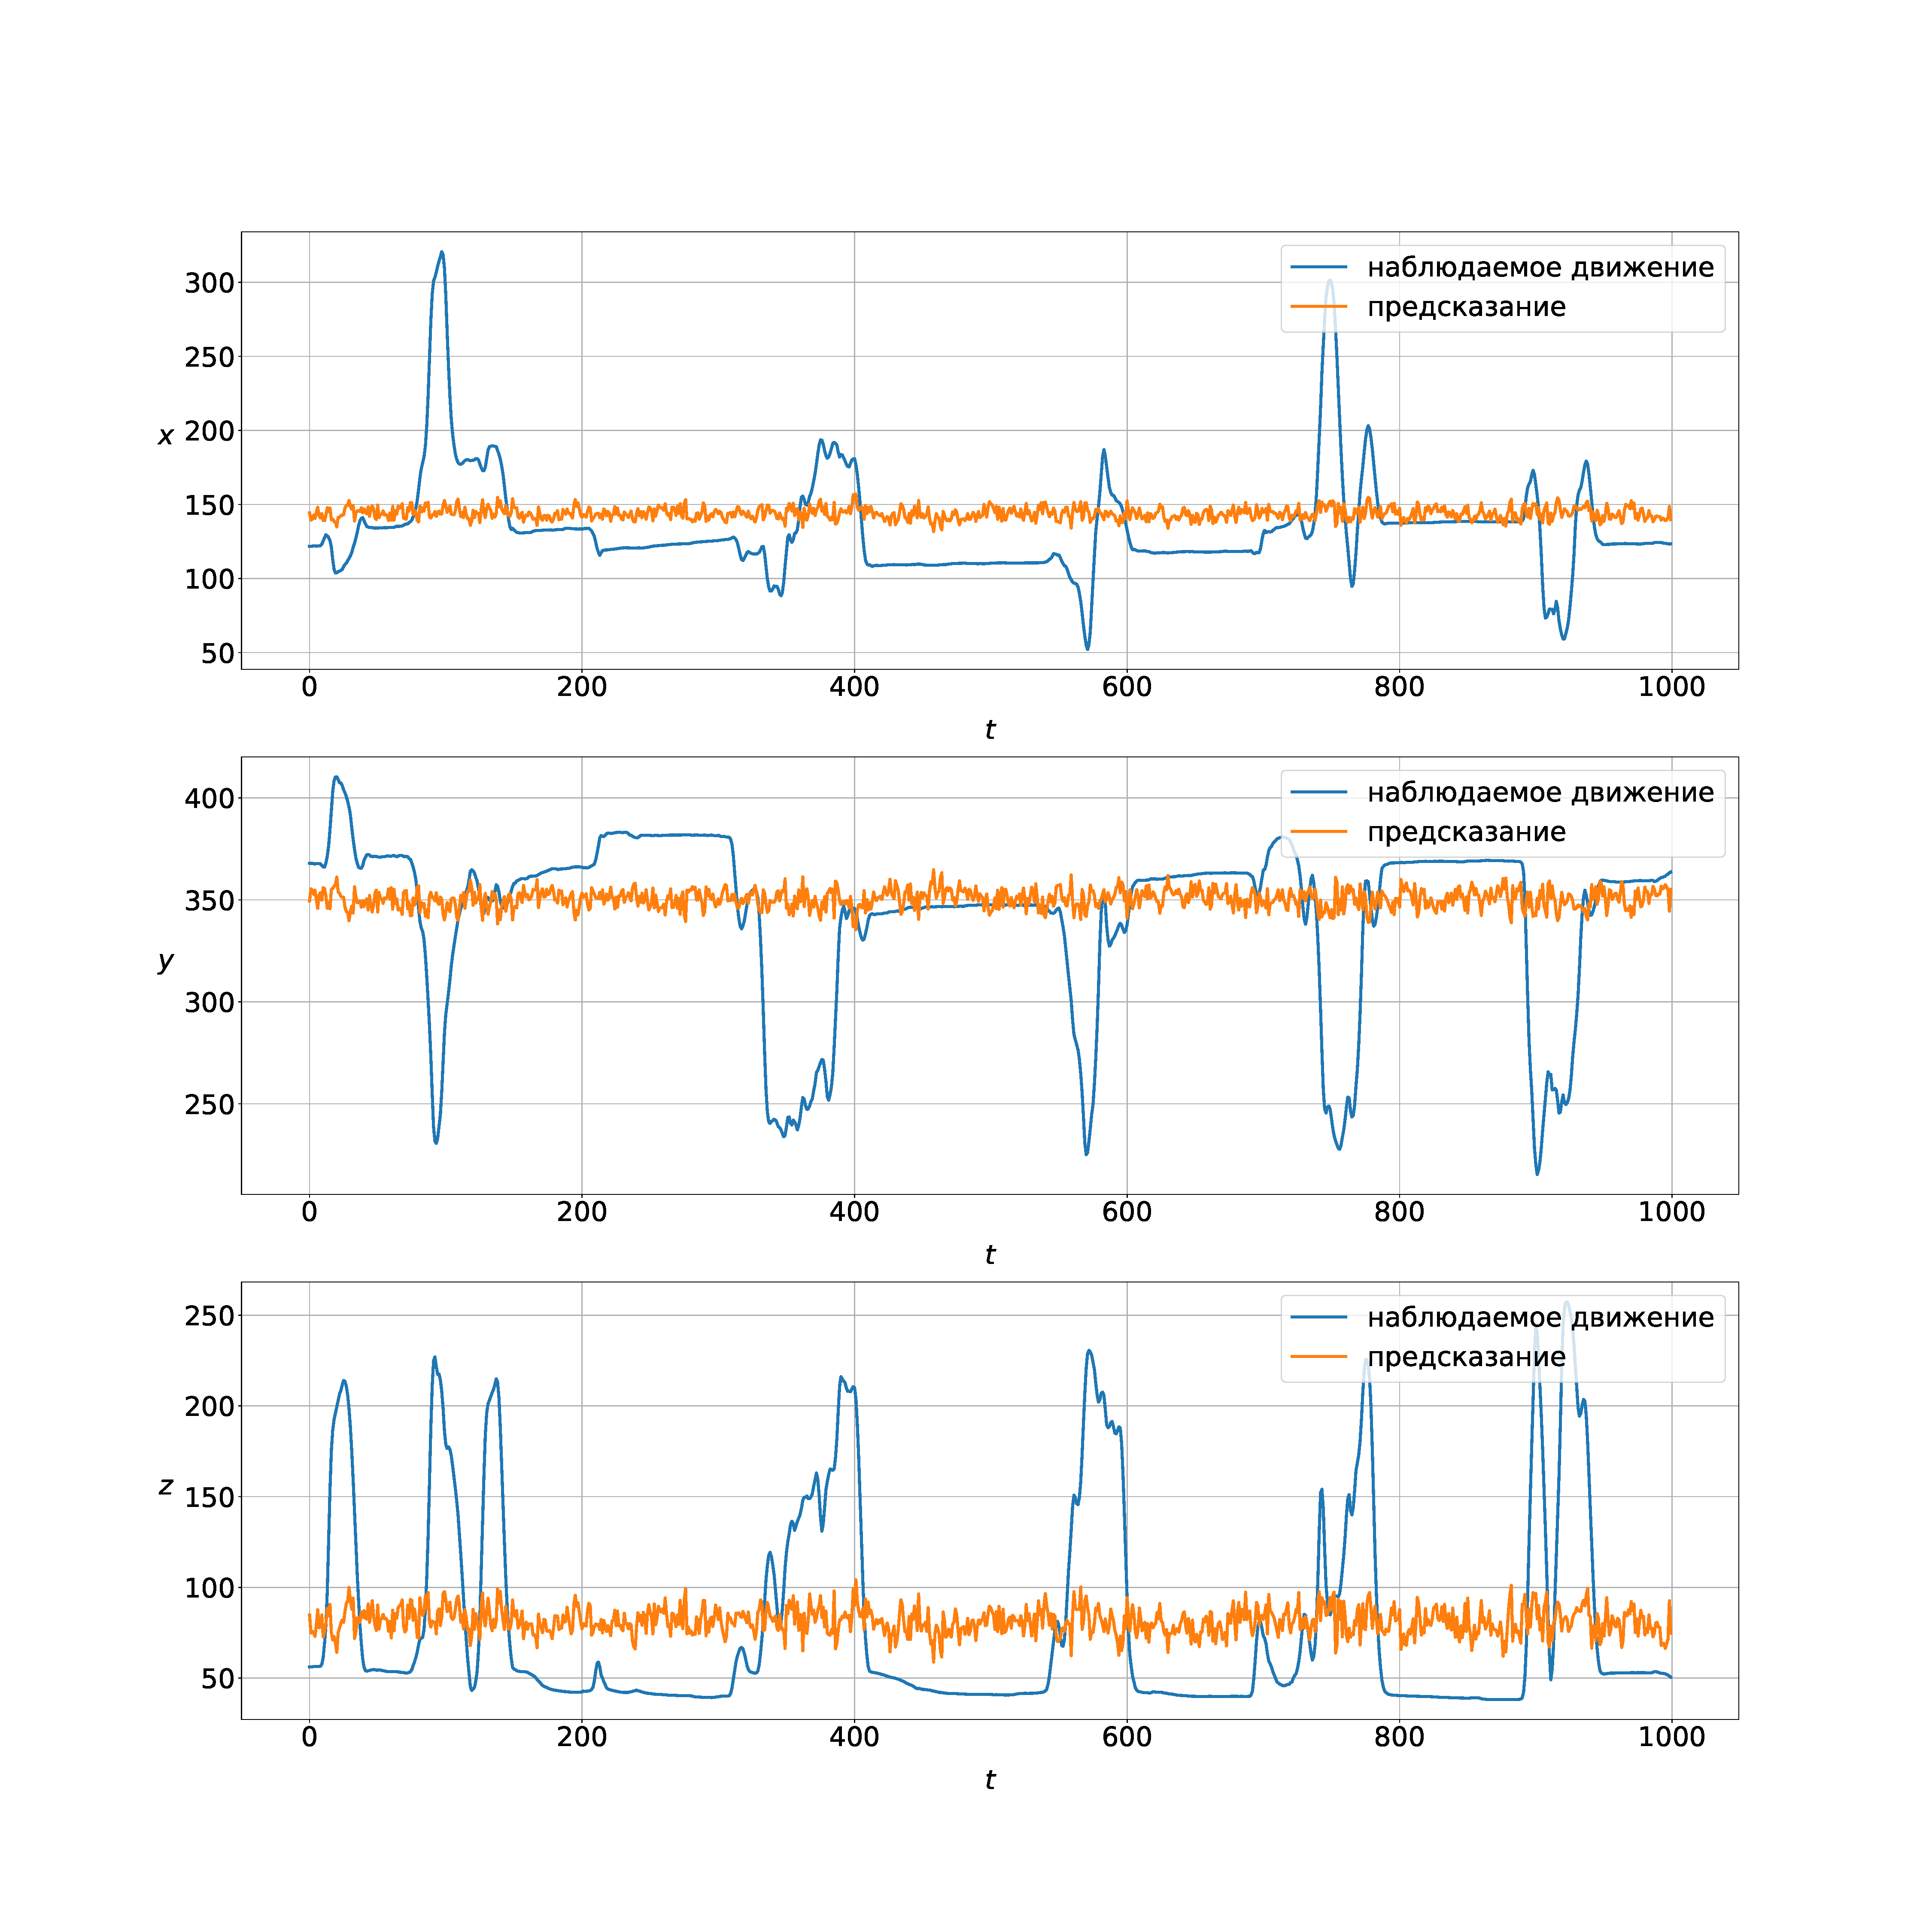
\includegraphics[width=\textwidth]{main_algo.pdf}
    \caption{Предсказания двухкомпонентного PLS, обученного на параметрах локальной модели}
    \label{fig:mainAlgo}
  \end{center}
\end{figure}
Как видно из рисунка, данная локальная модель плохо описывает исходные данные. Описать пики также не удалось. Избавиться от флуктуаций также не получилось. Эксперимент показал значения метрик $mae = 31.15, mse = 1908.62, r2 = -0.03$.

